\section{Introduction}
\label{sec:intro}

Operational logs from consumer IoT deployments record what each device did, when, and for
which account. They are long (an excerpt in our benchmark reaches $19{,}838$ tokens),
repetitive, and full of identifiers: account handles, device serials, contact fields. They
are also a natural substrate for question answering. An operator asks which device is
associated with a given account and expects a short answer.

The property that makes such a question answerable is also what makes it unsafe to send
verbatim. The question names an entity, and that entity is itself a protected value.
Redacting it before inference is the standard remedy, and it destroys the task: once the
account handle is gone, the model cannot tell which of two hundred similar records the
question refers to. Compressing the context is the other standard remedy, and it destroys
the task for a different reason. Under a redundancy-ordered rule the record carrying the
answer survives compression in $47.5\%$ of cases on our benchmark, and in only $37.2\%$ of
needle cases, where the answer value repeats across distractor records and the score gives it
no priority. Both remedies treat protecting the value and keeping the reference as competing
goals to be balanced.

\begin{figure*}[t]
\centering
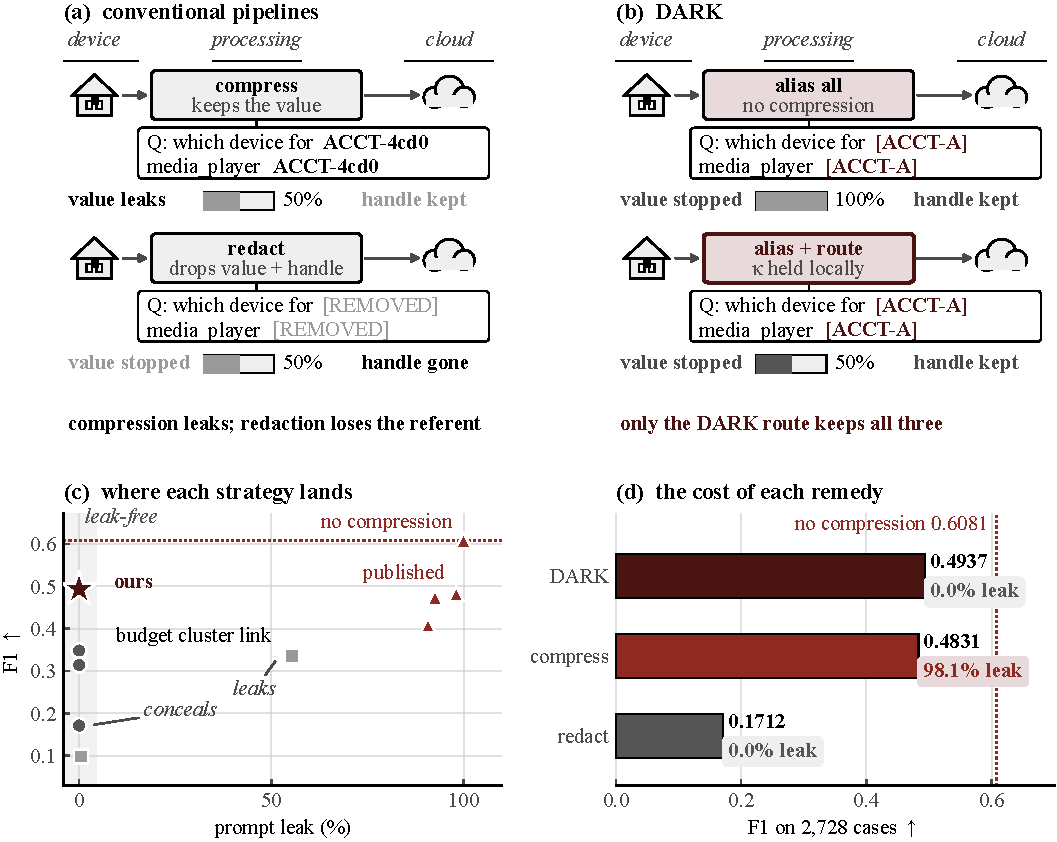
\includegraphics[width=\textwidth]{figures/fig0_teaser.pdf}
\caption{Three axes, four routes. Under each route the pale box is the prompt as the model
receives it---the rewritten question and the record line that carries the answer---and the bar
beside the badges is the share of the context that crosses; compressed routes run to the same
$r=0.50$ budget.
(a)~The conventional remedies. Compressing keeps the handle and halves the context, but
forwards the protected value, which the strongest such method leaves recoverable in $98.1\%$
of cases. Redacting removes the value and, with it, the handle the reader needs, so the
masking wrapper that does both loses the task. (b)~The two routes on our side. Aliasing every
protected value stops the value and keeps the handle, but does not compress.
\textsc{DARK} stops the value, keeps the handle, and fits the same budget. Only the fourth
route holds all three. (c)~F1 against prompt leakage for ten arms on the $2{,}728$-case
extension. The published compressors forward the value in $88.8\%$ to $100\%$ of cases, the
other leak-free arms land between $0.147$ and $0.348$, and only the marked point reaches
$0.494$ without leaking. (d)~The three policies on the same cases: \textsc{DARK} matches the
strongest published compressor on F1, but that arm forwards a protected value in $98.1\%$ of
cases, while the redaction baseline reaches $0\%$ leakage at $0.1712$.}
\label{fig:teaser}
\end{figure*}

For this class of query, they need not compete. Figure~\ref{fig:teaser} sets out three
axes---whether the protected value reaches the model, whether the handle the reader needs
survives, and how much of the context crosses. Compression and redaction both halve the
context, but compression forwards the value while redaction deletes the handle with it. A
fourth route, which we develop here, stops the value and keeps the handle at the same half
length.
The observation that makes this possible is a layout property. Records in these excerpts are
grouped into blocks that hold an entity's identifying
line together with the attributes recorded for it, so the queried entity and the answer to
the question about it sit in the \emph{same block} in every case, by construction. A pipeline that preserves that block, and replaces the protected
values inside it with stable aliases, keeps a referential handle while never exposing the
value. Finding the block requires no answer key: the question already names the entity, and
the block is whatever contains that mention.

\paragraph{What this implies for the design.}
A single global decision cannot express it. Aliasing every protected value keeps the handle
but spends budget on sensitive records that no question component will use; deleting every
protected value removes the handle along with the value. The two axes have to be decided per
unit, and the sensitive-and-relevant cell needs an operation that neither redaction nor
deletion provides. We therefore route each unit on the pair (sensitivity, relevance) and give
each cell its own operation. Sensitive and irrelevant units are \emph{deleted}. Irrelevant
insensitive units \emph{refill} whatever budget remains. Relevant insensitive units are
\emph{kept} verbatim. Sensitive-and-relevant units are \emph{aliased} rather than deleted.
The four operations give the method its name, \textsc{DARK}: \textbf{D}elete,
\textbf{A}lias, \textbf{R}efill, \textbf{K}eep.

\paragraph{Evidence preview.}
The design is judged against pipelines that keep the same privacy guarantee, because that is
the only comparison in which the privacy operation is held fixed. On a 112-case benchmark
spanning six public datasets, \textsc{DARK} uses $48.6\%$ of the original tokens, leaves no
protected value recoverable from the prompt, and scores F1 $0.6366$. Aliasing the whole
context without compressing it scores $0.6475$ on the same cases, a difference that is not
significant, so on this benchmark halving the prompt costs no measurable task quality. The
strongest leak-free competitor reaches $0.4308$, and in the multi-entity subset it still
exposes protected values. On a $2{,}728$-case extension, \textsc{DARK} is level with the best
query-aware compressor ($0.4937$ vs.\ $0.4831$) at $0\%$ leakage against $98.1\%$: the
compressor reaches the same F1 only by forwarding the value the question names, which is the
one thing this setting forbids. Removing the alias-instead-of-delete rule costs $0.1795$ F1
points overall and $0.3273$ on multi-entity cases. On the topical-question variant, where no
entity can be located, it costs $+0.0013$ and is not significant. The rule acts where it is
designed to act and is inert elsewhere.

\paragraph{Contributions.}
\begin{itemize}
\item \textbf{A failure mode that the compression literature does not report.} When the
queried entity is also the protected object, redundancy ordering carries almost no signal
about which record the question is about. We quantify it on $2{,}728$ cases ($47.5\%$
retention overall, $37.2\%$ on needle cases, both at a budget cut that would give an
uninformative rule $50\%$) and show that protecting the anchor \emph{line} alone repairs only
half of the gap ($57.6\%$).
\item \textbf{A training-free routing rule that closes the gap.} Sensitive-and-relevant units
are aliased rather than deleted, and relevance comes from the question by locating the record
block that contains the queried entity. The rule keeps a protected value addressable without
ever stating it, and needs no reference answer, no training, and no model access.
\item \textbf{An evaluation that separates privacy from utility at equal budget.} Across two
benchmark sizes, three public-benchmark variants, five budgets, two models, and two
paraphrases, \textsc{DARK} is compared with six published compressors re-run at full scale
plus a masking baseline and a 2026 rule-based compressor, with paired bootstrap
intervals on every difference we report. The
comparison is deliberately two-sided: at equal budget \textsc{DARK} is level with the best
query-aware compressor on F1 and $98.1$ points below it on leakage, and $+0.1456$
$[+0.1249,+0.1668]$ above the strongest leak-free arm, which differs from it only in which
region of the record survives.
\end{itemize}

Figure~\ref{fig:why} states the setting, the conflict it creates, and the position our rule
occupies in one view. Section~\ref{sec:related} positions the work; Section~\ref{sec:problem}
fixes notation and the threat model; Section~\ref{sec:method} presents the routing rule;
Sections~\ref{sec:benchmark}--\ref{sec:results} describe the benchmark and the results;
Section~\ref{sec:analysis} isolates each design decision; Section~\ref{sec:discussion}
states the scope the evidence supports.
